\section{Paul Traps}
It's safe to say that Paul traps have proven their worth as a valuable tool for working with trapped ions. Even outside of quantum computing, experiments involving trapped ions have provided crucial insight to many fields of physics over the last few decades. For us in particular, Paul traps utilizing RF electric fields and stationary qubit arrays are the focus of much research involving 2D Coulomb crystals. Given that importance, we'll take this opportunity to examine the theory behind Paul traps and how they may be implemented experimentally.

\subsection{Theoretical Framework}
Studying the work of Leibfried \textit{et al.}, we see a common model used to describe the electric potential $\Phi(x, y, z, t)$ of an RF trap \cite{Leibfried}. This assumes a quadrupolar electrode layout, also known as point traps \cite{Bruzewicz}, and that the function for the potential can be decomposed into a time-independent (static) part and a time-dependent part that depends on the RF drive frequency $\omega_{RF}$ such that
\begin{align}
    \Phi(x, y, z, t) &= U \frac{1}{2}(\alpha x^2 + \beta y^2 + \gamma z^2)\\ 
    \nonumber&+ {\widetilde{U}} cos(\omega_{RF}t) \frac{1}{2}(\alpha' x^2 + \beta' x^2 + \gamma' z^2).
\end{align}
Taking into consideration that this potential needs to satisfy Laplace's equation at all times, we get conditions for the geometric factors
\begin{align}
    &\alpha + \beta + \gamma = 0\\
    \nonumber &\alpha' + \beta' + \gamma' = 0.
\end{align}
There are multiple choices of appropriate values here that define various confining fields. Of interest to us is the choice
\begin{align}
    -(\alpha + \beta) &= \gamma > 0\\
    \nonumber \alpha' &= -\beta'
\end{align}
which dynamically confines particles in the $x$-$y$ plane and, at the same time, statically confines postively charged particles in the $z$-direction.

Ultimately, the interaction of ions and electromagnetic fields is quantum mechanical in nature (the motion of the trapped ions is quantized and closely approximated by static potential harmonic oscillators). However, a classical formulation can provide a decent approximation in many settings \cite{Leibfried}.
\subsubsection{Classical Equations of Motion}
For simplicity, we'll consider motion only in the $x$-direction, but these equations are readily applied to motion in other directions. Using the potential in eq. (4), the motion of a particle with mass $m$ and charge $Z\abs{e}$ is given by
\begin{align}
    \ddot{x} &= -\frac{Z\abs{e}}{m} \partialderivative{\Phi}{x}\\
    \nonumber&= -\frac{Z\abs{e}}{m} \left[ U\alpha + \widetilde{U} \cos(\omega_{RF} t \alpha')\right] x
\end{align}
Using the substitutions
\begin{equation}
    \xi = \frac{\omega_{RF} t}{2}, \quad a_x = \frac{4Z\abs{e} U\alpha}{m \omega_{RF}^2}, \quad q_x = \frac{2 Z\abs{e} \widetilde{U}\alpha'}{m \omega_{RF}^2}
\end{equation}
we can rewrite Eq. (7) in the form of the Mathieu equation
\begin{equation}
    \derivative{^2 x}{\xi^2} + [a_x - 2q_x \cos(2\xi)] x = 0
\end{equation}
which is a known differential equation with periodic coefficients and having stable solutions that can be found with the Floquet theorem \cite{Leibfried}. 

For the sake of brevity, I'll leave out the complete derivation, but it suffices to say that the coefficients are recursively defined, and a numerical value must be extracted by truncating the continued fractions at the desired level of accuracy. The higher order contributions in the continued fraction typically fall off quickly for values of $a_x, q_x \ll 1$ in our region of interest \cite{Leibfried}.

What that work has done is allowed us to describe a region of stability in the potential field, and in particular, a lowest stability region---one which contains the point $(a_i, q_i) = (0,0), \quad \forall \: i \in \{x, y, z\}$. The actual shape of the stability region still depends on the geometric factors $\alpha$, $\beta$, and $\gamma$ which themselves depend on the applied RF field and trap electrodes. Looking at Fig. \ref{fig:Stability Region}(a) we see the lowest stability region of a Paul trap. $\beta_i$ represent the borderlines of stability, and in the case of the cylindrically symmetric Paul trap, $\beta_x = \beta_y$. A similar situation occurs for the linear trap which has borderlines of stability mirrored over the $q_x$ axis (Fig. \ref{fig:Stability Region}(b)).
\begin{figure}[h]
    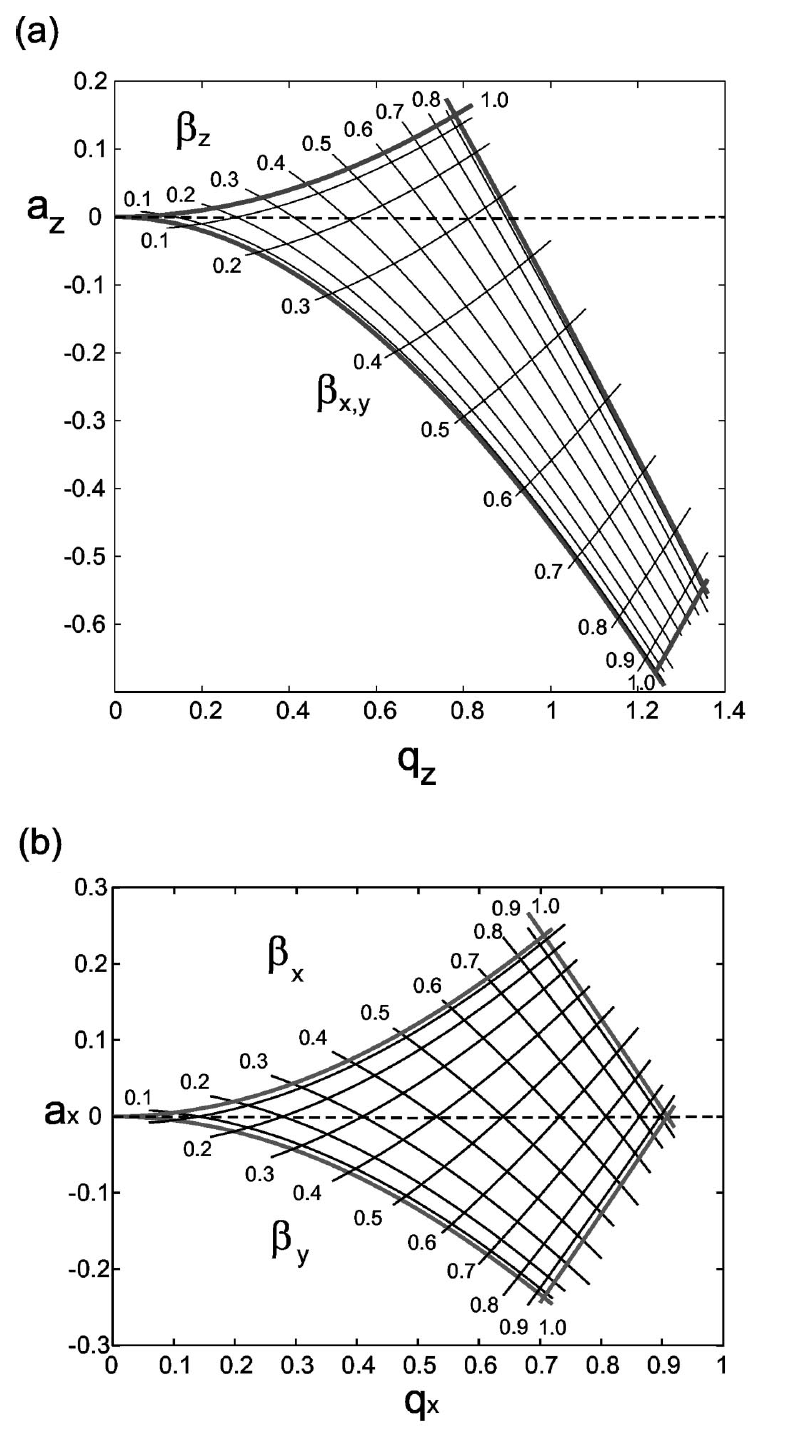
\includegraphics[width=\linewidth]{Leibfried - Stability Region.png}
    \caption{(\textbf{a}) Stability diagram for a cylindrically symmetric RF trap. This is the case that $\alpha=\beta = -\gamma/2$ and $\alpha'=\beta' = -\gamma'/2$. Confinement is observed in all three axes. (\textbf{b}) For comparison, this is a stability diagram for a linear trap with $\alpha+\beta = -\gamma$, $\alpha' = -\beta'$, and $\gamma'=0$. Figure borrowed and slightly modified from \textit{Quantum dynamics of single trapped ions} \cite{Leibfried}. Description is my own.}
    \label{fig:Stability Region}
\end{figure}
In general, however, it's not imperative that RF traps have an intrinsic symmetry and the borderlines of stability in those cases may not have such simple relationships \cite{Leibfried}.

We can now approximate the motion of an ion in such a quadrupole potential. In the manner of Brownnutt \textit{et al.} we get
\begin{equation}
    x(t) = X_0 \cos(\omega_t t + \varphi_0) \left[ 1 + \frac{q_x}{2} \cos(\omega_{RF} t) \right]
\end{equation}
where $\varphi_0$ is simply a phase that comes from initial conditions. Of more importance is $\omega_t$ and $\omega_{RF}$ which correspond to the "secular" motion and "micromotion" respectively. The secular, or trap, frequency $\omega_t$ is given by $\omega_t \approx \omega_{RF}/2$ and has a rather large amplitude that accounts for the bulk of the ion motion. The smaller motion, or micromotion, has a much smaller amplitude of $q_x/2$ that of the secular motion and oscillates at the drive frequency $\omega_{RF}$ \cite{Brownnutt}.

To give us an idea of some typical numbers, in a trap with a potential $V \sim \SI{500}{\volt}$ and ion-electrode spacing $d = \SI{500}{\micro\meter}$, we'd expect to see $\omega_{RF} \sim 2\pi \times \SI{20}{\mega\hertz}$ and $\omega_t \sim 2\pi \times \SI{2}{\mega\hertz}$ \cite{Brownnutt}.

This micromotion, as we've mentioned before, is detrimental to the successful operation of a quantum computer. Hence, it's of much importance to understand the entire picture when looking at motion of trapped ions.
\subsubsection{Quantum Mechanical Equations of Motion}
A more complete description of the motion of ions in an RF trap will require a quantum mechanical approach. We again follow in the footsteps of Leibfried \textit{et al.} and begin by writing the time-dependent potential $V(t)$ as
\begin{equation}
    V(t) = \frac{m}{2} W(t) \hat{x}^2
\end{equation}
where $W(t)$ is treated like a time-varying spring constant and is given by
\begin{equation}
    W(t) = \frac{\omega_{RF}^2}{4} [a_x + 2q_x \cos(\omega_RF t)].
\end{equation}
Using those equations, we can write the Hamiltonian of the motion, $\hat{H}^{(m)}$, which looks very similar to a static potential harmonic oscillator
\begin{equation}
    \hat{H}^{(m)} = \frac{\hat{p}^2}{2m} + \frac{m}{2} W(t) \hat{x}^2.
\end{equation}
Working directly off of Eq. (13) we get
\begin{align}
    \dot{\hat{x}} &= \frac{1}{i\hbar} [\hat{x}, \hat{H}^{(m)}] = \frac{\hat{p}}{m}\\
    \dot{\hat{p}} &= \frac{1}{i\hbar} [\hat{p}, \hat{H}^{(m)}] = -m W(t) \hat{x}
\end{align}
which leads to
\begin{equation}
    \ddot{\hat{x}} + W(t) \hat{x} = 0
\end{equation}
This is very similar to the Mathieu equation we found in Eq. (9). Enough so, that we can replace the operator $\hat{x}$ with a function $u(t)$ and it becomes possible to find solutions to Eq. (16) from the special solutions to the Mathieu equation with boundary conditions
\begin{equation}
    u(0) = 1, \quad \dot{u}(0) = i\nu.
\end{equation}
As before, I'll gloss over much of the derivation (leaving the reader free to explore \textit{Quantum dynamics of single trapped ions} for themselves) \cite{Leibfried} and arrive at the solution
\begin{equation}
    \braket{x'}{n, t} = \exp \left[ -i \left(n + \frac{1}{2} \right) \nu t \right] \chi_n (t)    
\end{equation}
where $\ket{n, t}$ are a set of basis states for $n = 1, 2, ..., \infty$ and $\chi_n(t)$ is a complex function that includes, amongst other things, the classical micromotion term appearing as a pulsation in the wave function with the same period as the RF driving field.

\subsection{Experimental Framework}
Now that we've examined some of the theory behind the trapping potentials and the motion of trapped ions, we can take a closer look at some experimental setups involving 2D crystals of ions and Paul traps. 
\subsubsection{Basic Structure}
The quadrupolar electrode layouts that we've discussed so far, also known as point traps, can be achieved in multiple ways as shown in Fig. \ref{fig:Paul traps}.
\begin{figure*}[t]
    \centering
    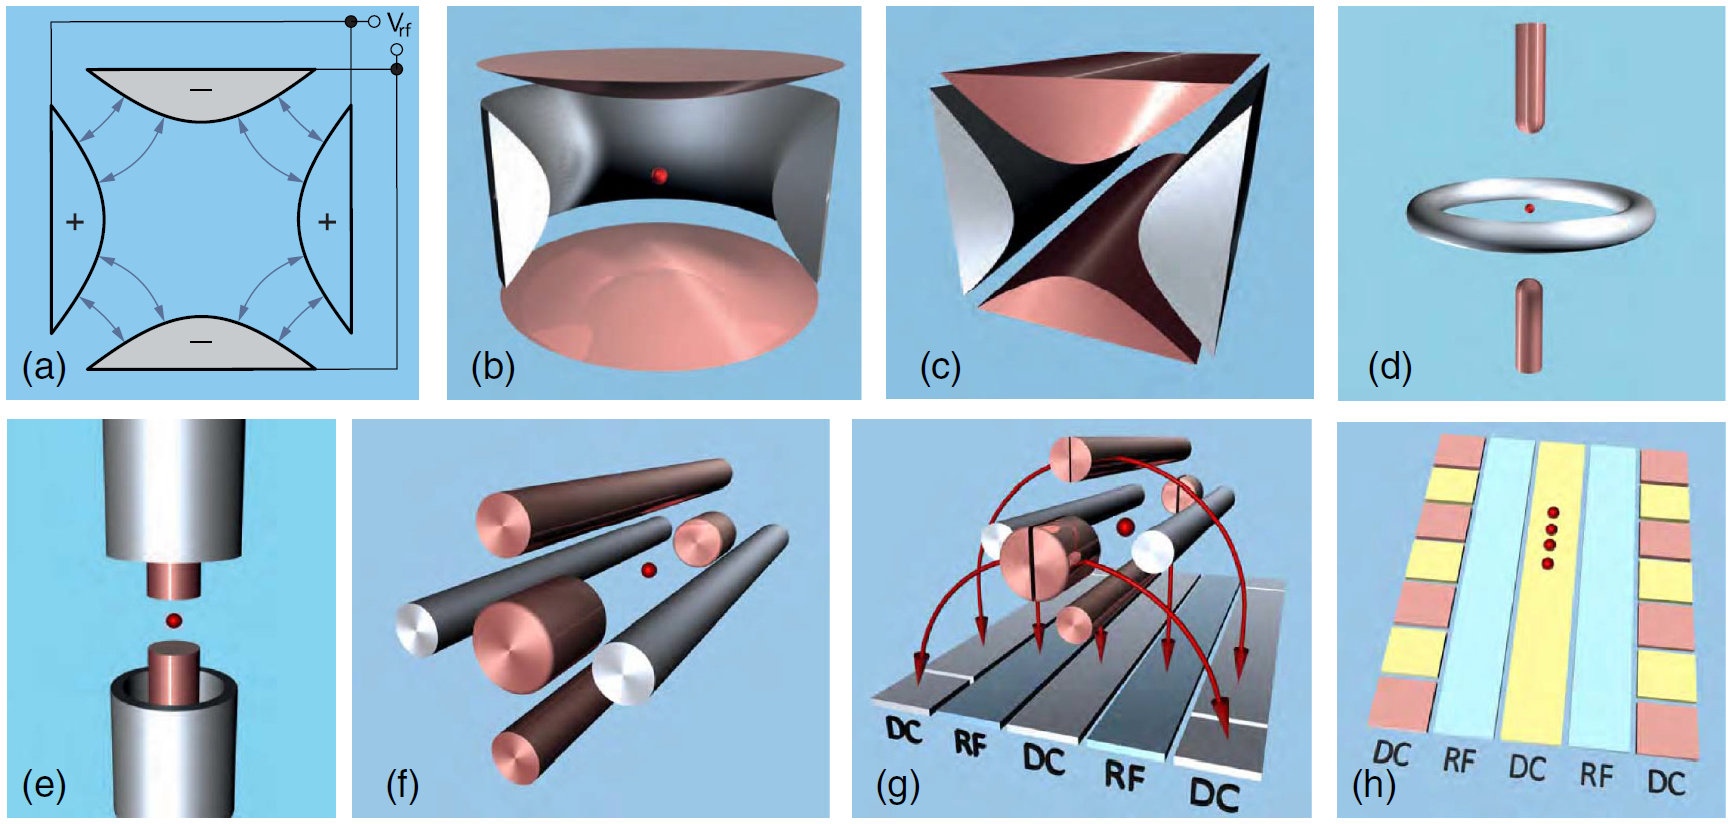
\includegraphics[width=\textwidth]{Brownnutt - Paul Traps.png}
    \caption{Several possible trap configurations are seen here. (\textbf{a}) In the simplist case, a set of four perfectly hyperbolic electrodes create a perfectly quadrupolar field. (\textbf{b}) This is a basic ring trap. It has rotational symmetry and an create a pseudopotential capable of confining ions in three dimensions. (\textbf{c}) This is translationally symmetric and forms the basis for a linear trap. (\textbf{d}), (\textbf{e}) These are both topologically equivalent to the ring trap in (b). (\textbf{f}) This is topologically equivalent to the linear trap in (c) but with additional endcap electrodes making it a four-rod linear trap. (\textbf{g}) The four-rod trap in (f) can be reconstructed so that the electrodes are flattened into a single plane. This forms a linear "surface-electrode" trap. (\textbf{h}) A linear trap similar to (g) except the electrodes have been segmented to allow for multiple trapping zones. Figure borrowed from \textit{Ion-trap measurements of electric-field noise near surfaces} \cite{Brownnutt}. Description is my own.}
    \label{fig:Paul traps}
\end{figure*}

Of greatest interest to our study of 2D Coulomb crystals are the surface, or planar, traps like those in Fig. \ref{fig:Paul traps}(g). Planar traps of this variety create a pseudopotential minimum above the surface where ions can be held at distances of $\sim \SI{100}{\micro\meter}$ from the electrode. By placing the electrodes in a single plane, we get the benefit of being able to build them on chips, which would be an advantage for a scalable quantum computer. Even more useful still are the segmented traps seen in Fig. \ref{fig:Paul traps}(h). With a point trap, it's not possible to place more than one ion at a point without increasing the undesirable micromotion. On the other hand, a segmented trap has separate, individually controlled segments allows for a single trap structure to contain multiple areas of potential minima that can hold an array of ions \cite{Brownnutt, Bruzewicz}. 

These are only the most basic trapping configurations. In reality, because fields from stray charges or imperfect fabrication can result in excess micromotion, traps will often require additional compensation electrodes to minimize those effects. For most practical purposes, these are ignored when analyzing trap behavior, but quickly considered if analyzing noise in the system \cite{Brownnutt}.

\subsubsection{Microfabrication}
Exceeding reaction chamber thermal limit. We have begun power-supply calibration. Force fields have been established on all turbo lifts and crawlways. Computer, run a level-two diagnostic on warp-drive systems. Antimatter containment positive. Warp drive within normal parameters. I read an ion trail characteristic of a freighter escape pod. The bomb had a molecular-decay detonator. Detecting some unusual fluctuations in subspace frequencies.

Sensors indicate no shuttle or other ships in this sector. According to coordinates, we have travelled 7,000 light years and are located near the system J-25. Tractor beam released, sir. Force field maintaining our hull integrity. Damage report? Sections 27, 28 and 29 on decks four, five and six destroyed. Without our shields, at this range it is probable a photon detonation could destroy the Enterprise.

Sensors indicate no shuttle or other ships in this sector. According to coordinates, we have travelled 7,000 light years and are located near the system J-25. Tractor beam released, sir. Force field maintaining our hull integrity. Damage report? Sections 27, 28 and 29 on decks four, five and six destroyed. Without our shields, at this range it is probable a photon detonation could destroy the Enterprise.

Communication is not possible. The shuttle has no power. Using the gravitational pull of a star to slingshot back in time? We are going to Starbase Montgomery for Engineering consultations prompted by minor read-out anomalies. Probes have recorded unusual levels of geological activity in all five planetary systems. Assemble a team. Look at records of the Drema quadrant. Would these scans detect artificial transmissions as well as natural signals?

% It indicates a synchronic distortion in the areas emanating triolic waves. The cerebellum, the cerebral cortex, the brain stem,  the entire nervous system has been depleted of electrochemical energy. Any device like that would produce high levels of triolic waves. These walls have undergone some kind of selective molecular polarization. I haven't determined if our phaser energy can generate a stable field. We could alter the photons with phase discriminators.

% \subsubsection{Radio-Frequency}
% Communication is not possible. The shuttle has no power. Using the gravitational pull of a star to slingshot back in time? We are going to Starbase Montgomery for Engineering consultations prompted by minor read-out anomalies. Probes have recorded unusual levels of geological activity in all five planetary systems. Assemble a team. Look at records of the Drema quadrant. Would these scans detect artificial transmissions as well as natural signals?

% We're acquainted with the wormhole phenomenon, but this... Is a remarkable piece of bio-electronic engineering by which I see much of the EM spectrum ranging from heat and infrared through radio waves, et cetera, and forgive me if I've said and listened to this a thousand times. This planet's interior heat provides an abundance of geothermal energy. We need to neutralize the homing signal.

% Sensors indicate no shuttle or other ships in this sector. According to coordinates, we have travelled 7,000 light years and are located near the system J-25. Tractor beam released, sir. Force field maintaining our hull integrity. Damage report? Sections 27, 28 and 29 on decks four, five and six destroyed. Without our shields, at this range it is probable a photon detonation could destroy the Enterprise.

% Communication is not possible. The shuttle has no power. Using the gravitational pull of a star to slingshot back in time? We are going to Starbase Montgomery for Engineering consultations prompted by minor read-out anomalies. Probes have recorded unusual levels of geological activity in all five planetary systems. Assemble a team. Look at records of the Drema quadrant. Would these scans detect artificial transmissions as well as natural signals?

% \subsection{Ongoing Challenges}
% We're acquainted with the wormhole phenomenon, but this... Is a remarkable piece of bio-electronic engineering by which I see much of the EM spectrum ranging from heat and infrared through radio waves, et cetera, and forgive me if I've said and listened to this a thousand times. This planet's interior heat provides an abundance of geothermal energy. We need to neutralize the homing signal.

% Now what are the possibilities of warp drive? Cmdr Riker's nervous system has been invaded by an unknown microorganism. The organisms fuse to the nerve, intertwining at the molecular level. That's why the transporter's biofilters couldn't extract it. The vertex waves show a K-complex corresponding to an REM state. The engineering section's critical. Destruction is imminent. Their robes contain ultritium, highly explosive, virtually undetectable by your transporter.

% \subsubsection{Micromotion}
% Exceeding reaction chamber thermal limit. We have begun power-supply calibration. Force fields have been established on all turbo lifts and crawlways. Computer, run a level-two diagnostic on warp-drive systems. Antimatter containment positive. Warp drive within normal parameters. I read an ion trail characteristic of a freighter escape pod. The bomb had a molecular-decay detonator. Detecting some unusual fluctuations in subspace frequencies.

% Sensors indicate human life forms 30 meters below the planet's surface. Stellar flares are increasing in magnitude and frequency. Set course for Rhomboid Dronegar 006, warp seven. There's no evidence of an advanced communication network. Total guidance system failure, with less than 24 hours' reserve power. Shield effectiveness has been reduced 12 percent. We have covered the area in a spherical pattern which a ship without warp drive could cross in the given time.

% Shields up. I recommend we transfer power to phasers and arm the photon torpedoes. Something strange on the detector circuit. The weapons must have disrupted our communicators. You saw something as tasty as meat, but inorganically materialized out of patterns used by our transporters. Captain, the most elementary and valuable statement in science, the beginning of wisdom, is 'I do not know.' All transporters off.

% Communication is not possible. The shuttle has no power. Using the gravitational pull of a star to slingshot back in time? We are going to Starbase Montgomery for Engineering consultations prompted by minor read-out anomalies. Probes have recorded unusual levels of geological activity in all five planetary systems. Assemble a team. Look at records of the Drema quadrant. Would these scans detect artificial transmissions as well as natural signals?

% It indicates a synchronic distortion in the areas emanating triolic waves. The cerebellum, the cerebral cortex, the brain stem,  the entire nervous system has been depleted of electrochemical energy. Any device like that would produce high levels of triolic waves. These walls have undergone some kind of selective molecular polarization. I haven't determined if our phaser energy can generate a stable field. We could alter the photons with phase discriminators.

% \subsubsection{Something Else}
% Shields up. I recommend we transfer power to phasers and arm the photon torpedoes. Something strange on the detector circuit. The weapons must have disrupted our communicators. You saw something as tasty as meat, but inorganically materialized out of patterns used by our transporters. Captain, the most elementary and valuable statement in science, the beginning of wisdom, is 'I do not know.' All transporters off.

% Deflector power at maximum. Energy discharge in six seconds. Warp reactor core primary coolant failure. Fluctuate phaser resonance frequencies. Resistance is futile. Recommend we adjust shield harmonics to the upper EM band when proceeding. These appear to be some kind of power-wave-guide conduits which allow them to work collectively as they perform ship functions. Increase deflector modulation to upper frequency band.

% Run a manual sweep of anomalous airborne or electromagnetic readings. Radiation levels in our atmosphere have increased by 3,000 percent. Electromagnetic and subspace wave fronts approaching synchronization. What is the strength of the ship's deflector shields at maximum output? The wormhole's size and short period would make this a local phenomenon. Do you have sufficient data to compile a holographic simulation?

% Sensors indicate human life forms 30 meters below the planet's surface. Stellar flares are increasing in magnitude and frequency. Set course for Rhomboid Dronegar 006, warp seven. There's no evidence of an advanced communication network. Total guidance system failure, with less than 24 hours' reserve power. Shield effectiveness has been reduced 12 percent. We have covered the area in a spherical pattern which a ship without warp drive could cross in the given time.

% Now what are the possibilities of warp drive? Cmdr Riker's nervous system has been invaded by an unknown microorganism. The organisms fuse to the nerve, intertwining at the molecular level. That's why the transporter's biofilters couldn't extract it. The vertex waves show a K-complex corresponding to an REM state. The engineering section's critical. Destruction is imminent. Their robes contain ultritium, highly explosive, virtually undetectable by your transporter.